% !TEX root = ./Basilisk-MODULENAME-yyyymmdd.tex

\section{Model Description}

\begin{figure}[H]
	\centerline{
		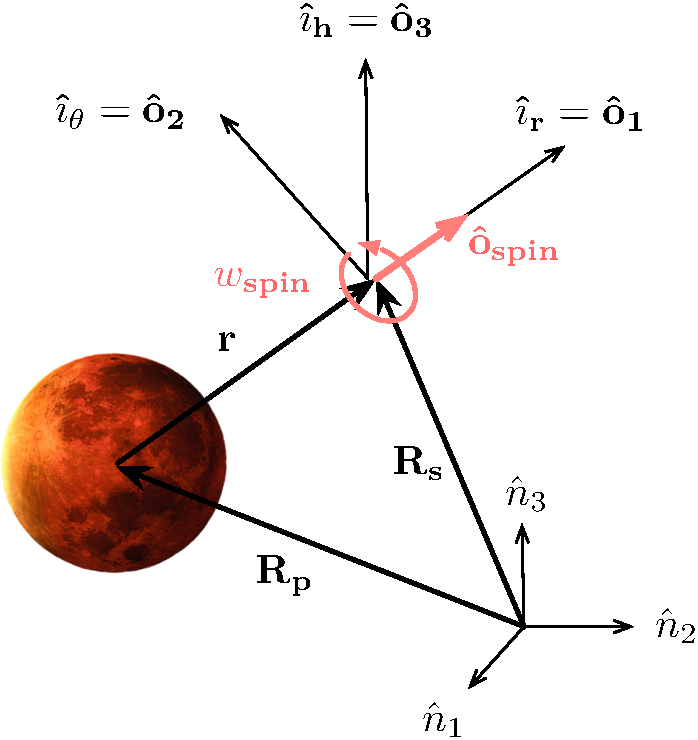
\includegraphics{Figures/Fig1}
	}
	\caption{Sample Figure Inclusion.}
	\label{fig:Fig1}
\end{figure}

The sunline ephemeris module is responsible for calculating a sunline heading based exclusively on ephemeris data. This provides a estimate for the sun heading without relying of filtering results from the course sun sensors. 

Describe the module including mathematics, implementation, etc.

\subsection{Equations}
Equations are centered with the equation number flush to the right. In the text, these equations should be referenced by name as Eq.~\eqref{eq:ab} or Equation~\eqref{eq:ab} (e.g., not eq.  1, (1), or Equation 1).
\begin{equation}
	\hat{r_{h_N}} = \frac{r_{sc} - r_{sun}}{|r_{sc} - r_{sun}|}
\end{equation}

\begin{equation}
	\hat{r}_{h_B} = DCM_{BN}*\hat{r}_{h_N}
\end{equation}

